%%%%%%%%%%%%%%%%%%%%%%%%%%%%%%%%%%%%%%%%%%%%%%%%%%%%%%%%%%%%%%%%%%%%%%
%     File: ExtendedAbstract_resul.tex                               %
%     Tex Master: ExtendedAbstract.tex                               %
%                                                                    %
%     Author: Andre Calado Marta                                     %
%     Last modified : 27 Dez 2011                                    %
%%%%%%%%%%%%%%%%%%%%%%%%%%%%%%%%%%%%%%%%%%%%%%%%%%%%%%%%%%%%%%%%%%%%%%
% Results
% Results should be clear and concise.
% Discussion
% This should explore the significance of the results of the work, not
% repeat them. A combined Results and Discussion section is often
% appropriate. Avoid extensive citations and discussion of published
% literature.
%%%%%%%%%%%%%%%%%%%%%%%%%%%%%%%%%%%%%%%%%%%%%%%%%%%%%%%%%%%%%%%%%%%%%%

\section{Results}
\label{sec:resul}

This section will focus in testing and comparing the control algorithm developed so far, with and without the online NN corrections. These results will mainly focus in comparing both performances when facing modelling errors and system failures.


%%%%%%%%%%%%%%%%%%%%%%%%%%%%%%%%%%%%%%%%%%%%%%%%%%%%%%%%%%%%%%%%%%%%%%
\subsection{Inversion Errors}

This error will be the most frequent when implementing such a controller, as some system parameters estimations may have considerable errors, namely the aircraft inertial matrix. Fortunately, the controller used is, as it will be demonstrated, tolerant to errors in the estimation of this parameter, but can result in an unstable system in extreme cases. To simulate estimation errors, the entries of the inertial matrix $I_{xx}$,$I_{yy}$,$I_{zz}$ and $I_{xz}$ were multiplied by a reducing factor $\zeta \in [0;1]$ when computing the nonlinear inversion in \ref{eq:control_law}. The inertial matrix used in this equation $I_{est}$ is therefore given by $I_{est} = \zeta I$.

In order to more accurately visualise the influence of the $\zeta$ coefficient on the NLI controller for this same case, several simulations were made for values of $\zeta$ from $0$ to $1$. For each simulation the mean error was computed, in order to obtain a plot of these errors for each of the three references. From Figure \ref{fig:xi_mean_error} can be concluded that the error becomes considerable $\zeta<0.05$ for a controller without neural network compensation. For a compensated adaptive controller however, it is noticeable that errors only become considerable at $\zeta<0.02$.

\begin{figure}[h]
\centering
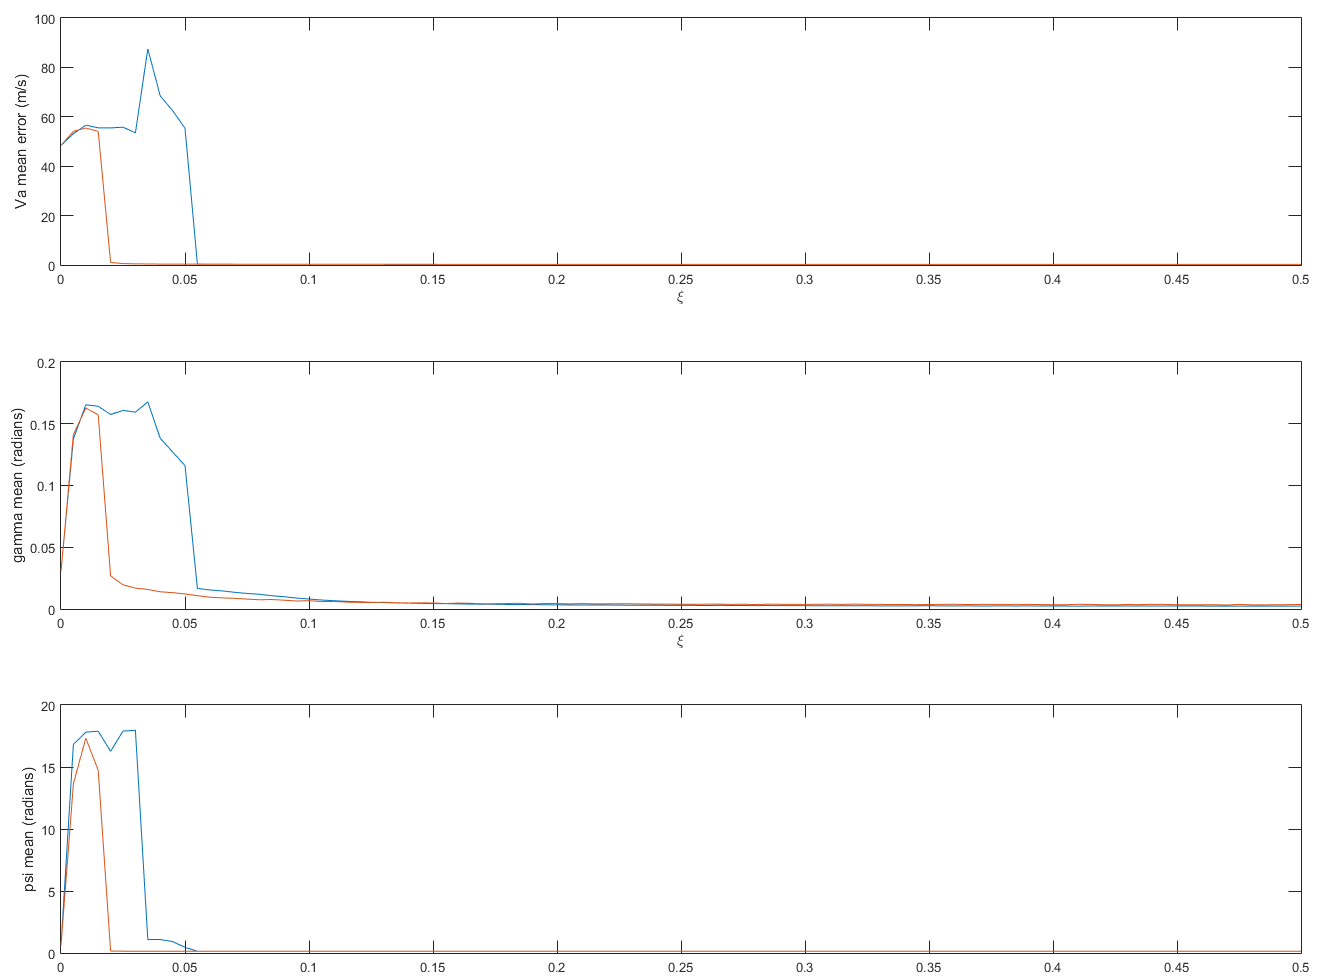
\includegraphics[width=0.5\textwidth]{../Figures/Results/mean_error_xi.png}
\caption[Mean errors for $V_a$, $\gamma$ and $psi$]{Mean errors for $V_a$, $\gamma$ and $psi$ for $\zeta=[0,0.5]$ with neural network compensation (orange) and without compensation (blue)}
\label{fig:xi_mean_error}
\end{figure}

\begin{figure}[h]
\centering
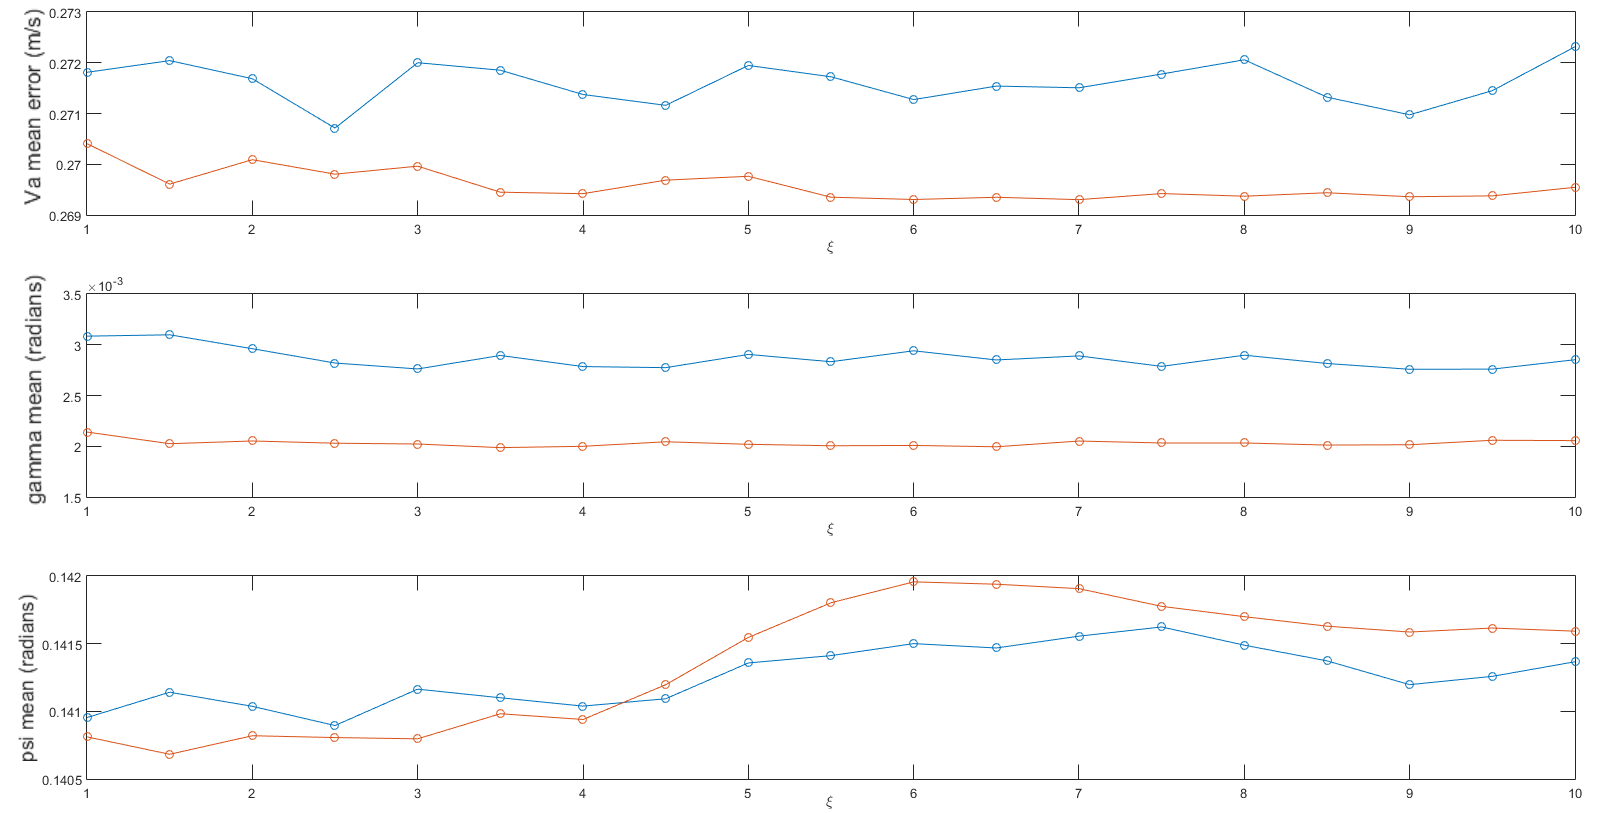
\includegraphics[width=0.5\textwidth]{../Figures/Results/mean_error_xi_big.png}
\caption[Mean errors for $V_a$, $\gamma$ and $psi$ for larger values of $\zeta$ ]{Mean errors for $V_a$, $\gamma$ and $psi$ for $\zeta=[1,10]$ with neural network compensation (orange) and without compensation (blue)}
\label{fig:xi_mean_error_big}
\end{figure}

Although the errors showed in figure \ref{fig:xi_mean_error_big} are small and almost neglectable for these values of $\zeta$, these results still show, for $\gamma$ and $V_a$, the NN is capable of reducing the mean error when compared to the non corrected controller. This one however is able to perform correctly with a small tracking error for larger values of $\zeta$.

\subsection{System Failures and External Disturbances}

One other cause for inversion errors that can have a much greater impact on flight trajectory are system failures.  The reference trajectory that will be used shall be the same as used previously. The first failure to be simulated will be a control surfaces failure, that will lead to reduced controllability of the aircraft. In this work this was replicated in a simulated environment by reducing by 80\% each moment coefficients for the elevator, aileron and rudder, namely $C_{\delta_{ele}}$, $C_{\delta_{ail}}$ and $C_{\delta_{rud}}$.

Applying the adaptive correction through the online neural network, the following trajectories were obtained

\begin{figure}[h]
\centering
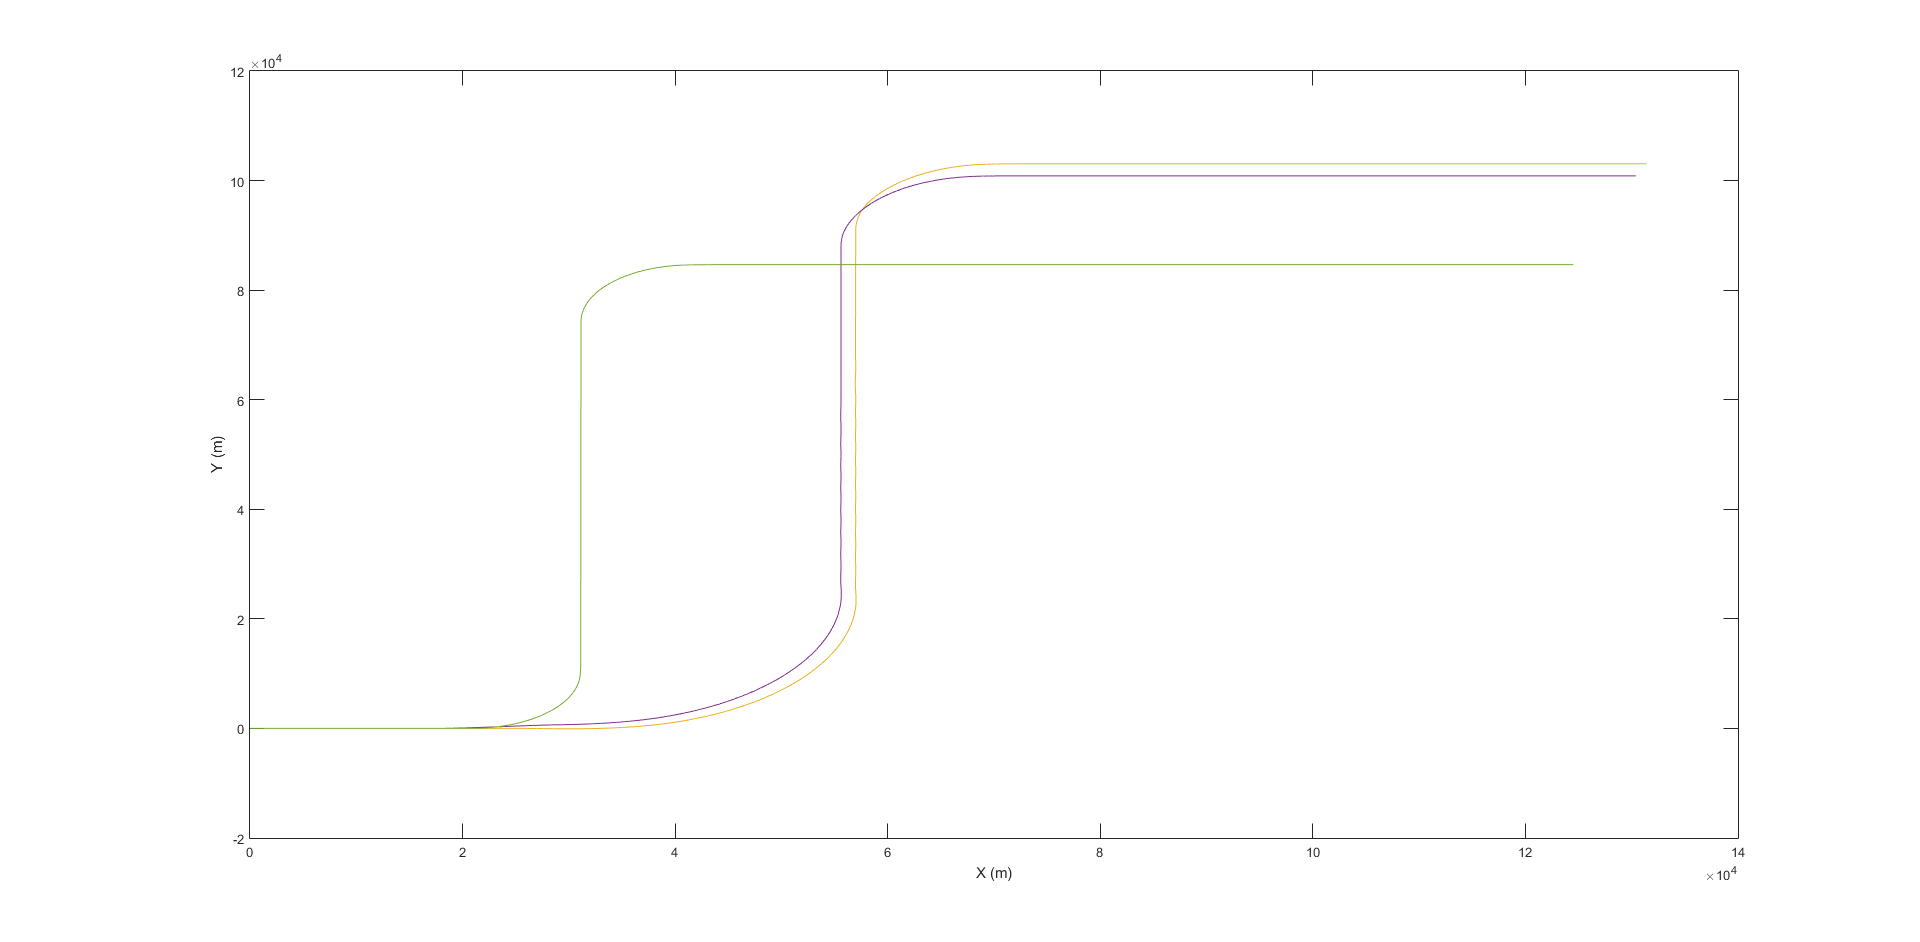
\includegraphics[width=0.5\textwidth]{../Figures/Results/reduced_act_NN.png}
\caption[Trajectory with reduced actuation corrected with NN correction]{Trajectory with 20\% reduced actuation (yellow) and trajectory without failures (green). The corrected trajectory by the NN can be seen in purple}
\label{fig:reduced_act_NN}
\end{figure}

The first observation that can be drawn from figure \ref{fig:reduced_act_NN} is that such an actuator failure severely reduces the controllability of the aircraft. 

The main consequence for this case will be, as could be expected, an increase in the convergence time to the desired heading. Note that the desired trajectory is not followed as this correction is only applied to the fast dynamics, and a guidance control law is not used. Comparing the two cases where the failures were implemented however, it can be observed that system corrected by the neural network converged to the desired heading slightly faster, resulting in a $2000m$ reduction in distance when comparing the non corrected control trajectory. 

One second type of flight perturbation that was studied is the effects of icing conditions in aircraft flight. According to the FAA guide to flight in icing conditions, ice contamination of an airfoil has an important influence on both the Lift and Drag curves, according to the \cite{icing_cond}.

\begin{itemize}
\item \textbf{Stall }Ice contamination of the airfoil leads to a significant reduction in the value of the maximum $C_L$, causing the aircraft to reach stall conditions at a much lower angle of attack. Reducing speed (e.g for an approach) makes this effect more noticeable for the pilot. The usual reduction on $C_{L_{max}}$ is of 30\% \cite{icing_cond}.

\item \textbf{Drag }Drag will increase directly with the amount of ice accumulated on the wing, reaching usual values of 100\% of the initial drag coefficient.

\item \textbf{Roll }Icing on the main wings will also affect roll control. As the thickness of the wing decreases towards its tip, so increases its efficiency to collect ice, leading to a partial stall in the tip of the wings, according to the AOPA manual \cite{icing_aopa}.
\end{itemize}

Following these indications to simulate heavy icing condition, the lift coefficient $C_{L_{max}}$ was reduced by 30\%, and the stall angle reduced to $15^o$. The value of the drag coefficient was also augmented by 200\%. Finally, in order to simulate roll control limitations, the value of $C_{\delta_{ail}}$ was reduced by 30\%. These values were chosen in order to deteriorate the control of the aircraft, while allowing for the possibility of reference following without reaching actuator saturation (for both control surface deflections and thrust). 

For this case a sinusoidal yaw reference was given of $\psi^d= 45 \sin (1.1459t)$ degrees, $t$ being the simulation time. A sinusoidal reference was used to make the effects of simulated icing more noticeable, and the airspeed and FPA references of $V_a^d=200ms^{-1}$ and $\gamma^d=0$ . For this case, the results obtained were as follows

\begin{figure}[h]
\centering
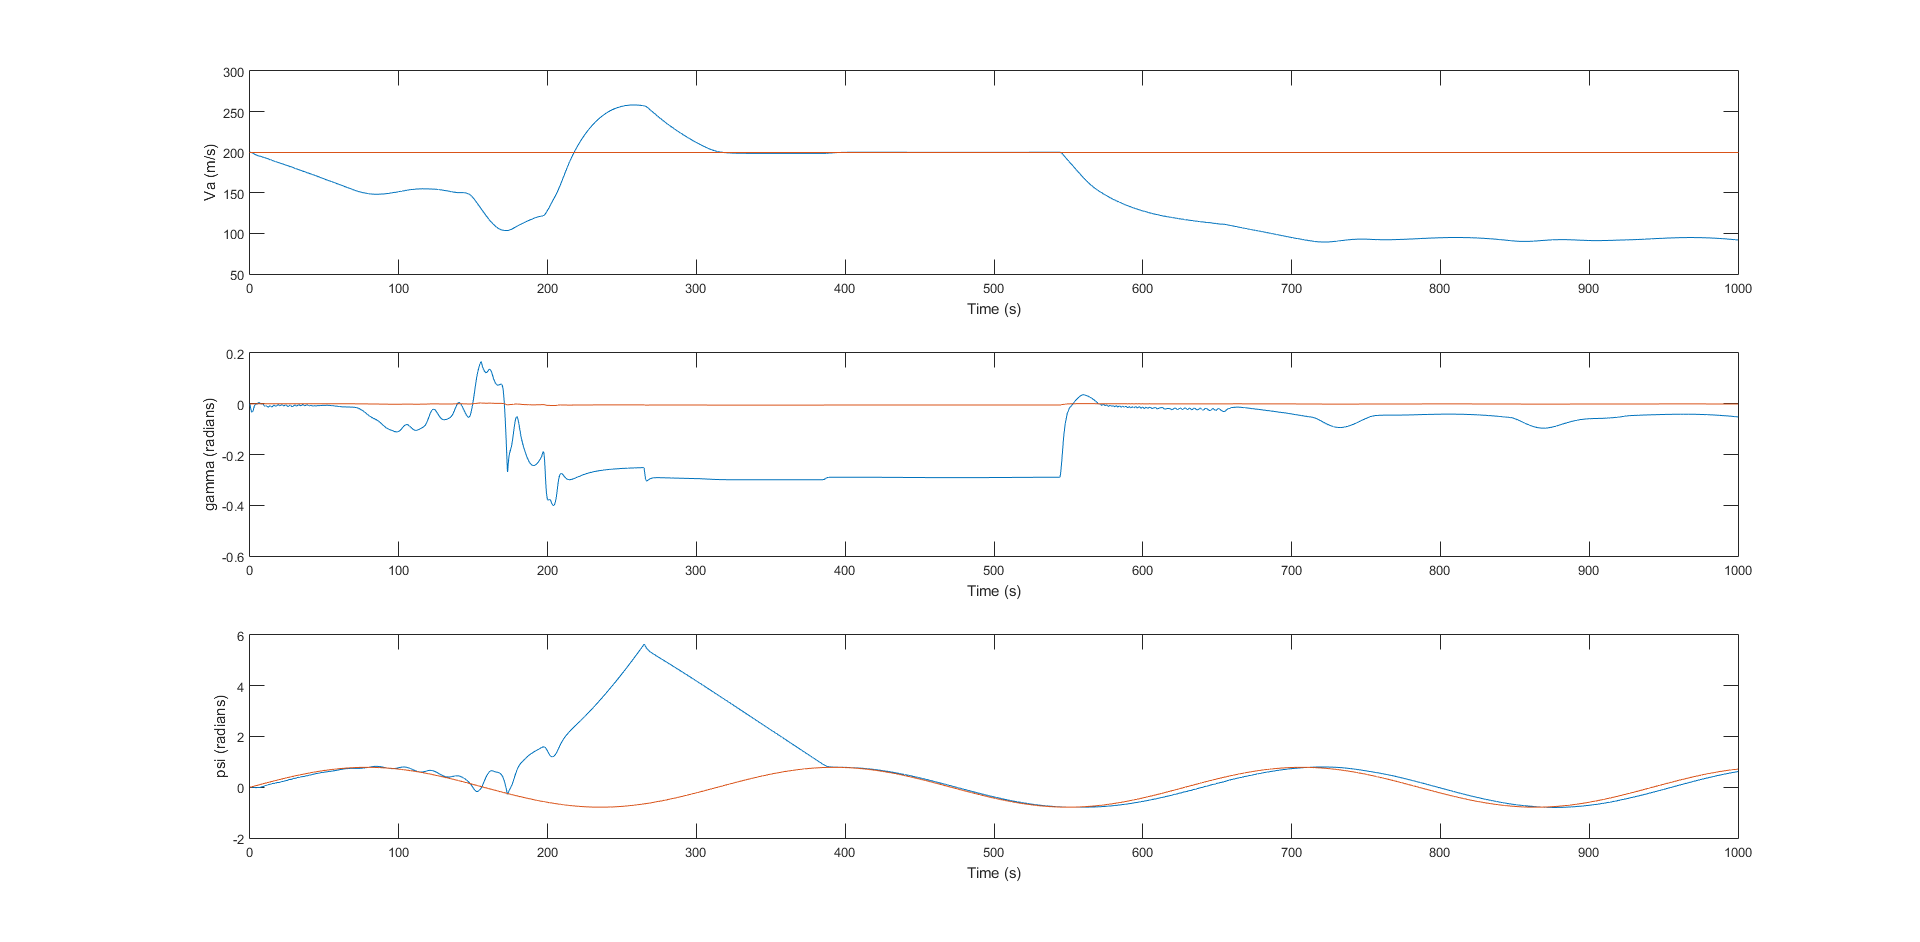
\includegraphics[width=0.5\textwidth]{../Figures/Results/ref_icing.PNG}
\caption[Reference following in icing conditions]{$V_a$, $\gamma$ and $\psi$ for measured and desired values in icing conditions without NN correction}
\label{fig:ref_icing}
\end{figure}

\begin{figure}[h]
\centering
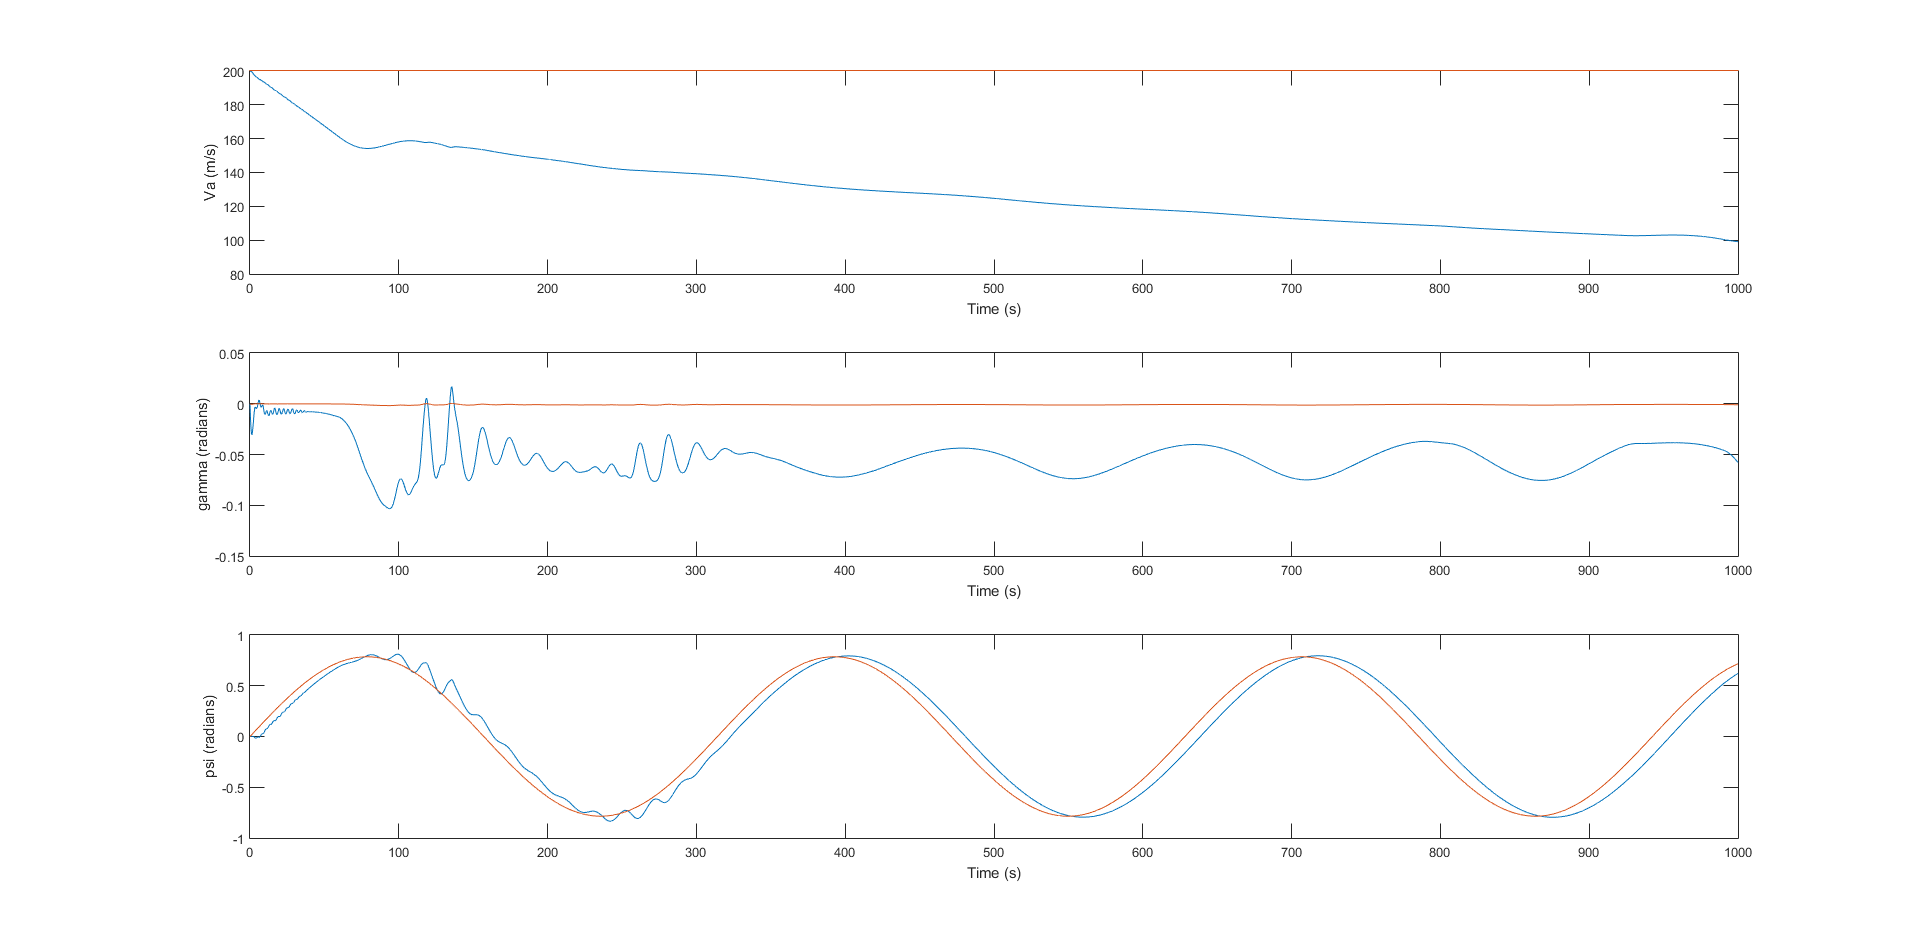
\includegraphics[width=0.5\textwidth]{../Figures/Results/ref_icing_NN.PNG}
\caption[Reference following in icing conditions with NN correction]{$V_a$, $\gamma$ and $\psi$ for measured and desired values in icing conditions with NN correction}
\label{fig:ref_icing_NN}
\end{figure}

From figure \ref{fig:ref_icing}, the system in such high drag conditions can be considered marginally stable, as it easily increases the error to either of the three commanded inputs to significantly high values. For the case of the flight path angle, the aircraft even reaches under $-20º$ at $t=600s$, a completely unrealistic value for a normal cruise flight. The impact of the increased drag in noticeable in the reduced speed in the simulation, going under $100ms^{-1}$ for the desired $V_a^d=200ms^{-1}$. The reduced roll capabilities and lift also cause errors and oscillations in heading and flight path angle following.

In Figure \ref{fig:ref_icing_NN}, the aircraft shows a more stable behaviour and smaller tracking errors. Again, these are conditions that have a negative impact on the controllability of the aircraft: the increase of 200\% of the value of $C_D$ causes a decrease in the speed of the aircraft, rendering it unable to follow the desired speed of $200ms^{-1}$. Regarding the measured flight path angle $\gamma$, although  some oscillations are still present, error relative to the reference no longer goes up to $0.3 rad$, instead oscillating around $0.05rad$ at a much lower frequency and amplitude. The most noticeable improvement however can be seen in the heading following: the aircraft follows the desired $\psi^d$ during the full simulation, with little to no oscillations around the desired value. It is also interesting to notice that in the first moments of the learning process, up to $t=300s$, oscillations around the desired heading value are greater than in later moments of the simulation. This is explained by the fact that the weights of the neural network have not yet converged to their optimal values at $t<300s$.
